\chapter{Introduktion}
I denne rapport dokumentere vi designet, implementation og evaluering af et snake spil. Snake spillet er det velkendte spil fra for exemple Nokia 3310 \cite{wiki_snake}. 

Formålet med projektopgaven er at genskabe det klassiske spil Snake, samt at dokumentere hvordan vi opbygger spillet. Spillet laves i to versioner: Simpel Snake og Avanceret Snake. Det skrives i Java.

Simpel Snake er en primitiv version af spillet, se \figref{simplesnake}. Styring og bevægelse foregår kun vha. input fra spilleren. Det bruges som udgangspunkt for den avancerede udgave.

I Avanceret Snake er der tilføjet forskellige funktioner, som enten forbedrer brugerfladen eller ændre på hvordan spillet spilles. For eksempel tilføjelse af hovedmenu og automatisk bevægelse af slangen, se \figref{advancedsnake}. Vi har udvidet det så to personer kan spille mod hinanden.

I rapporten vil designet og implementeringen af begge spillets versioner blive forklaret. I evaluerings kapitlerne redegør vi for tanker, valg og komplikationen som vi stødte på under projektet. 

\begin{figure}
	\centering
	\subfloat[Simpel Snake]{\figlab{simplesnake}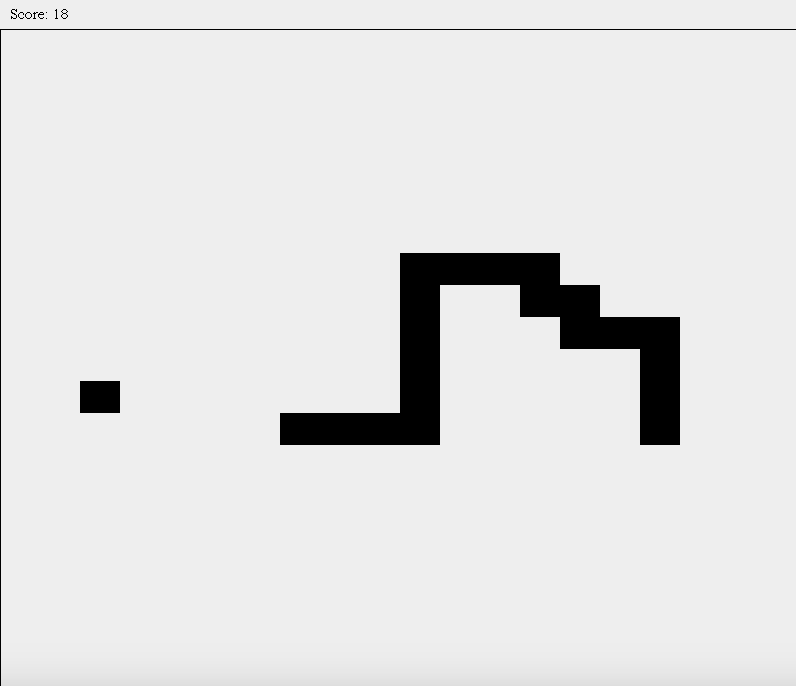
\includegraphics[width=0.43\textwidth]{SimpelSnake.png}}
	\hspace{0.1\textwidth}
	\subfloat[Avanceret Snake]{\figlab{advancedsnake}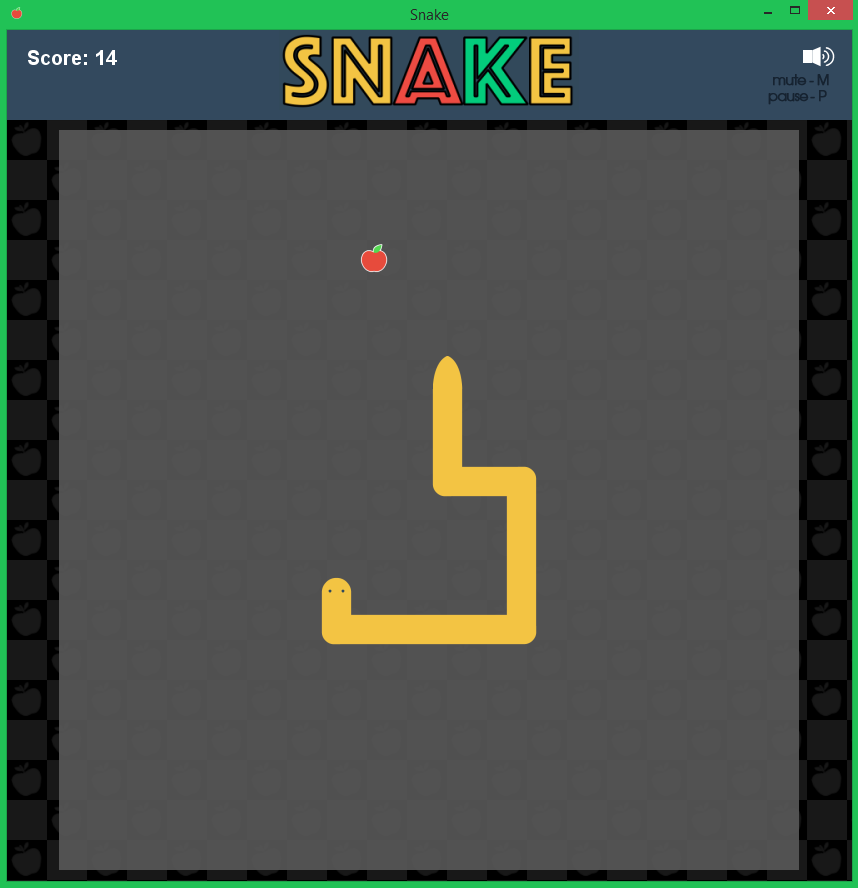
\includegraphics[width=0.46\textwidth]{AdvancedSnake.png}}
	\caption{Billede af Simpel og Avanceret Snake.}
\end{figure}